
% Second Stasheff identity using trees, with signs



\begin{center}
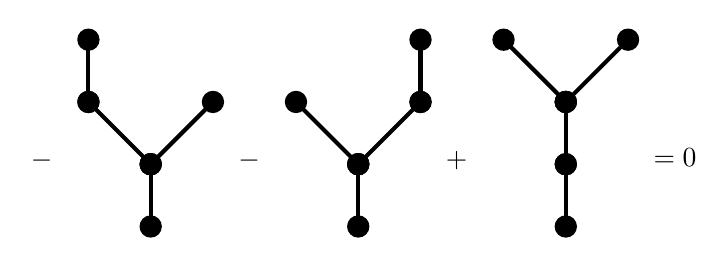
\begin{tikzpicture}[x=0.75pt,y=0.75pt,yscale=-1,xscale=1]
%uncomment if require: \path (0,300); %set diagram left start at 0, and has height of 300

%Straight Lines [id:da31477124000159296] 
\draw [line width=1.5]    (120,140) -- (90,110) ;
\draw [shift={(90,110)}, rotate = 225] [color={rgb, 255:red, 0; green, 0; blue, 0 }  ][fill={rgb, 255:red, 0; green, 0; blue, 0 }  ][line width=1.5]      (0, 0) circle [x radius= 4.36, y radius= 4.36]   ;
\draw [shift={(120,140)}, rotate = 225] [color={rgb, 255:red, 0; green, 0; blue, 0 }  ][fill={rgb, 255:red, 0; green, 0; blue, 0 }  ][line width=1.5]      (0, 0) circle [x radius= 4.36, y radius= 4.36]   ;
%Straight Lines [id:da49139183729214175] 
\draw [line width=1.5]    (120,140) -- (150,110) ;
\draw [shift={(150,110)}, rotate = 315] [color={rgb, 255:red, 0; green, 0; blue, 0 }  ][fill={rgb, 255:red, 0; green, 0; blue, 0 }  ][line width=1.5]      (0, 0) circle [x radius= 4.36, y radius= 4.36]   ;
\draw [shift={(120,140)}, rotate = 315] [color={rgb, 255:red, 0; green, 0; blue, 0 }  ][fill={rgb, 255:red, 0; green, 0; blue, 0 }  ][line width=1.5]      (0, 0) circle [x radius= 4.36, y radius= 4.36]   ;
%Straight Lines [id:da49681202435755245] 
\draw [line width=1.5]    (120,170) -- (120,140) ;
\draw [shift={(120,140)}, rotate = 270] [color={rgb, 255:red, 0; green, 0; blue, 0 }  ][fill={rgb, 255:red, 0; green, 0; blue, 0 }  ][line width=1.5]      (0, 0) circle [x radius= 4.36, y radius= 4.36]   ;
\draw [shift={(120,170)}, rotate = 270] [color={rgb, 255:red, 0; green, 0; blue, 0 }  ][fill={rgb, 255:red, 0; green, 0; blue, 0 }  ][line width=1.5]      (0, 0) circle [x radius= 4.36, y radius= 4.36]   ;
%Straight Lines [id:da3941708866613911] 
\draw [line width=1.5]    (220,140) -- (190,110) ;
\draw [shift={(190,110)}, rotate = 225] [color={rgb, 255:red, 0; green, 0; blue, 0 }  ][fill={rgb, 255:red, 0; green, 0; blue, 0 }  ][line width=1.5]      (0, 0) circle [x radius= 4.36, y radius= 4.36]   ;
\draw [shift={(220,140)}, rotate = 225] [color={rgb, 255:red, 0; green, 0; blue, 0 }  ][fill={rgb, 255:red, 0; green, 0; blue, 0 }  ][line width=1.5]      (0, 0) circle [x radius= 4.36, y radius= 4.36]   ;
%Straight Lines [id:da300120384085371] 
\draw [line width=1.5]    (220,140) -- (250,110) ;
\draw [shift={(250,110)}, rotate = 315] [color={rgb, 255:red, 0; green, 0; blue, 0 }  ][fill={rgb, 255:red, 0; green, 0; blue, 0 }  ][line width=1.5]      (0, 0) circle [x radius= 4.36, y radius= 4.36]   ;
\draw [shift={(220,140)}, rotate = 315] [color={rgb, 255:red, 0; green, 0; blue, 0 }  ][fill={rgb, 255:red, 0; green, 0; blue, 0 }  ][line width=1.5]      (0, 0) circle [x radius= 4.36, y radius= 4.36]   ;
%Straight Lines [id:da14962304311021435] 
\draw [line width=1.5]    (220,170) -- (220,140) ;
\draw [shift={(220,140)}, rotate = 270] [color={rgb, 255:red, 0; green, 0; blue, 0 }  ][fill={rgb, 255:red, 0; green, 0; blue, 0 }  ][line width=1.5]      (0, 0) circle [x radius= 4.36, y radius= 4.36]   ;
\draw [shift={(220,170)}, rotate = 270] [color={rgb, 255:red, 0; green, 0; blue, 0 }  ][fill={rgb, 255:red, 0; green, 0; blue, 0 }  ][line width=1.5]      (0, 0) circle [x radius= 4.36, y radius= 4.36]   ;
%Straight Lines [id:da6955709488854369] 
\draw [line width=1.5]    (320,110) -- (290,80) ;
\draw [shift={(290,80)}, rotate = 225] [color={rgb, 255:red, 0; green, 0; blue, 0 }  ][fill={rgb, 255:red, 0; green, 0; blue, 0 }  ][line width=1.5]      (0, 0) circle [x radius= 4.36, y radius= 4.36]   ;
\draw [shift={(320,110)}, rotate = 225] [color={rgb, 255:red, 0; green, 0; blue, 0 }  ][fill={rgb, 255:red, 0; green, 0; blue, 0 }  ][line width=1.5]      (0, 0) circle [x radius= 4.36, y radius= 4.36]   ;
%Straight Lines [id:da11504103913241726] 
\draw [line width=1.5]    (320,110) -- (350,80) ;
\draw [shift={(350,80)}, rotate = 315] [color={rgb, 255:red, 0; green, 0; blue, 0 }  ][fill={rgb, 255:red, 0; green, 0; blue, 0 }  ][line width=1.5]      (0, 0) circle [x radius= 4.36, y radius= 4.36]   ;
\draw [shift={(320,110)}, rotate = 315] [color={rgb, 255:red, 0; green, 0; blue, 0 }  ][fill={rgb, 255:red, 0; green, 0; blue, 0 }  ][line width=1.5]      (0, 0) circle [x radius= 4.36, y radius= 4.36]   ;
%Straight Lines [id:da004089317473789711] 
\draw [line width=1.5]    (320,140) -- (320,110) ;
\draw [shift={(320,110)}, rotate = 270] [color={rgb, 255:red, 0; green, 0; blue, 0 }  ][fill={rgb, 255:red, 0; green, 0; blue, 0 }  ][line width=1.5]      (0, 0) circle [x radius= 4.36, y radius= 4.36]   ;
\draw [shift={(320,140)}, rotate = 270] [color={rgb, 255:red, 0; green, 0; blue, 0 }  ][fill={rgb, 255:red, 0; green, 0; blue, 0 }  ][line width=1.5]      (0, 0) circle [x radius= 4.36, y radius= 4.36]   ;
%Straight Lines [id:da8569365387106636] 
\draw [line width=1.5]    (90,110) -- (90,80) ;
\draw [shift={(90,80)}, rotate = 270] [color={rgb, 255:red, 0; green, 0; blue, 0 }  ][fill={rgb, 255:red, 0; green, 0; blue, 0 }  ][line width=1.5]      (0, 0) circle [x radius= 4.36, y radius= 4.36]   ;
\draw [shift={(90,110)}, rotate = 270] [color={rgb, 255:red, 0; green, 0; blue, 0 }  ][fill={rgb, 255:red, 0; green, 0; blue, 0 }  ][line width=1.5]      (0, 0) circle [x radius= 4.36, y radius= 4.36]   ;
%Straight Lines [id:da41279118247571556] 
\draw [line width=1.5]    (250,110) -- (250,80) ;
\draw [shift={(250,80)}, rotate = 270] [color={rgb, 255:red, 0; green, 0; blue, 0 }  ][fill={rgb, 255:red, 0; green, 0; blue, 0 }  ][line width=1.5]      (0, 0) circle [x radius= 4.36, y radius= 4.36]   ;
\draw [shift={(250,110)}, rotate = 270] [color={rgb, 255:red, 0; green, 0; blue, 0 }  ][fill={rgb, 255:red, 0; green, 0; blue, 0 }  ][line width=1.5]      (0, 0) circle [x radius= 4.36, y radius= 4.36]   ;
%Straight Lines [id:da5701552758066648] 
\draw [line width=1.5]    (320,170) -- (320,140) ;
\draw [shift={(320,140)}, rotate = 270] [color={rgb, 255:red, 0; green, 0; blue, 0 }  ][fill={rgb, 255:red, 0; green, 0; blue, 0 }  ][line width=1.5]      (0, 0) circle [x radius= 4.36, y radius= 4.36]   ;
\draw [shift={(320,170)}, rotate = 270] [color={rgb, 255:red, 0; green, 0; blue, 0 }  ][fill={rgb, 255:red, 0; green, 0; blue, 0 }  ][line width=1.5]      (0, 0) circle [x radius= 4.36, y radius= 4.36]   ;

% Text Node
\draw (361,131.4) node [anchor=north west][inner sep=0.75pt]    {$=0$};
% Text Node
\draw (61,132.4) node [anchor=north west][inner sep=0.75pt]    {$-$};
% Text Node
\draw (161,132.4) node [anchor=north west][inner sep=0.75pt]    {$-$};
% Text Node
\draw (261,132.4) node [anchor=north west][inner sep=0.75pt]    {$+$};


\end{tikzpicture}    
\end{center}